\documentclass[twocolumns]{emulateapj}
%apj gives the referee version/preprint2
%\usepackage[T1]{fontenc}
%\usepackage[utf8]{inputenc}
%\usepackage{graphicx}
%\usepackage{natbib}
\usepackage{amsmath}
\usepackage{amssymb}
%\usepackage{vmargin}
%\usepackage{pdfpages}
\usepackage{aas_macros}


\usepackage[normalem]{ulem}
\usepackage[usenames]{color}

\definecolor{DarkGreen}{rgb}{0.64,0.80,0.35}
\newcommand\ALc[1]{{\color{red} \bf #1}} %Astrid
\newcommand\Ac[1]{{\color{green} \bf #1}} %% Avery
\newcommand\Pc[1]{{\color{cyan} \bf #1}} %% Phil
\newcommand\Cc[1]{{\color{blue} \bf #1}} %% Christoph
\newcommand\Ec[1]{{\color{magenta} \bf #1}} %% Ewald

\begin{document}
\title{How uniform is TeV-blazar heating?}

\author{Astrid Lamberts$^1$, Philip Chang$^1$, Ewald Puchwein$^2$, Christoph Pfrommer$^3$, Avery E. Broderick$^{4,5}$ and Mohamad Shalaby$^{2,3,6}$}
\affil{$^1$ Department of Physics, University of Wisconsin-Milwaukee, 1900 East Kenwood Boulevrad, Milwaukee WI 53211, USA}
\affil{$^2$ Institute of Astronomy and Kavli Institute for Cosmology, University of Cambridge, Madingley Road, Cambridge, CB3 0HA, UK}
\affil{$^3$ Heidelberg Institute for Theoretical Studies, Schloss-Wolfsbrunnenweg 35, D-69118 Heidelberg, Germany}
\affil{$^4$ Perimeter Institute for Theoretical Physics, 31 Caroline Street North, Waterloo, ON, N2L 2Y5, Canada}
\affil{$^5$ Department of Physics and Astronomy, University of Waterloo, 200 University Avenue West, Waterloo, ON, N2L 3G1, Canada}
\affil{$^6$ Department of Physics, Faculty of Science, Cairo University, Giza 12613, Egypt}
\email{lambera@uwm.edu}

%\altaffiltex{1}{Physics Department, UWM, Milwaukee WI 53211}

\begin{abstract}
TeV-blazars heat up the intergalactic medium (IGM) as the gamma-rays they produce turn into pairs which lose their kinetic energy to the surrounding medium through plasma instabilities.  Assuming uniform heating, this mechanism increases the temperature of the IGM and produces an inverted temperature-density relation in underdense regions. This additional heating source significantly impacts large scale structure formation. In this paper we go beyond the approximation of uniform heating and quantify the heating rate fluctuations and their impact on the thermal history of the IGM. We analytically compute a filtering function relating the heating rate fluctuations to the underlying  dark matter density field. We implement it in the cosmological code GADGET-3 and perform large scale simulations to determine the impact of inhomogeneous heating. We show that, because of the bias, blazar heating is inhomogeneous, at all redshifts. The temperature-density relation shows an important scatter and presents a low temperature envelope of unheated regions. However, the median temperature of the IGM is close to that in the uniform case, albeit slightly lower at low redshift. We find that blazar heating is more complex than initially assumed and that the temperature-density relation is not unique. Future work will deal with the observational impact and large scale structure formation in this context.  Our analytic model for the heating rate fluctuations couples well with large scale simulations and provides a cost-effective alternative to subgrid models.
\end{abstract}

\keywords{BL Lacertae objects: general, cosmology: theory, gamma-rays: genereal, intergalactic medium, large-scale structure of universe}
\section{Introduction}
The intergalactic medium is an ionized medium which relates galaxies and clusters together, thus forming the cosmic web \citep{1996Natur.380..603B}. It constitutes the main reservoir of baryons available for the formation of collapsed objects such as galaxies and clusters \citep{1997ApJ...489....7R}. Observations of metal-enriched materials (see e.g. \citet{2009A&A...493..409S,2010MNRAS.407.2063W}) prove its evolution due to already formed stars and galaxies. This close relation between the IGM and structure evolution makes it a  crucial aspect for the understanding of large scale structure in the universe.

The temperature of the IGM is mostly set by photoionization of hydrogen  and helium, competing with adiabatic cooling. This yields a slowly cooling universe, with denser regions being warmer because more resistant to adiabatic cooling. Observations of absorption lines in spectra of background quasars due to neutral gas confirm this equation of state \citep{2000MNRAS.318..817S,2000ApJ...534...41R,2012ApJ...757L..30R}. However, recent measurements found that underdense regions may be warmer than expected \citep{2009MNRAS.399L..39V,2008MNRAS.386.1131B,2014MNRAS.441.1916B}. Although an inverted temperature-density relation in underdense regions has not been firmly established yet \citep{2014MNRAS.tmp...52B}, the recent observations suggest the thermal history of the IGM is be more complex than initially assumed.



\citet{2012ApJ...752...22B} recently described a complementary heating mechanism, through TeV blazars. TeV blazars are active galactic nuclei emitting  very high energy gamma rays (E$\ge$100 GeV). About 50 of these sources have been discovered so far (http://tevcat.uchicago.edu/), by the space-based \textit{Fermi}/LAT and ground based Cerenkov telescopes such as MAGIC, H.E.S.S. and VERITAS. The universe is mainly opaque to  very high energy  gamma rays, as they interact with the extragalactic background light (EBL) producing electron/positron pairs \citep{1967PhRv..155.1408G,1992ApJ...390L..49S}.  It is commonly assumed that the electron/positron pairs then upscatter photons of the cosmic microwave background, resulting in  a halo of photons with energies between $.1$ and $100$ GeV. Such extended emission around TeV blazars has not been observed so far \citep{2010A&A...524A..77A,2014arXiv1401.2915H}, which is interpreted by deviations due to the intergalactic magnetic field (IGMF) \citep{2013A&ARv..21...62D,2012ApJ...747L..14V,2011ApJ...733L..21D}. \citet{2012ApJ...752...22B} showed that the pair beams rather transfer their energy directly to the IGM through plasma instabilities.

The pairs constitute a dilute, ultrarelativistic beam, which is subject to several plasma instabilities, from which the ``oblique'' instability \citep{PhysRevE.70.046401} is the most powerful. Assuming its efficiency in the linear regime extends to the non-linear regime, \citet{2012ApJ...752...23C} (hereafter PaperI) show it is responsible for increasing the temperature of the IGM by almost a factor 10 in low density regions. While this assumption is still debated (see \citet{2013ApJ...770...54M,2014ApJ...787...49S} but also \citet{2013arXiv1311.6752S,2013ApJ...777...49S,2012ApJ...758..102S}, Chang et al, submitted), throughout all this paper we will assume plasma instabilities are the dominant mechanism for cooling of the pair beams.


Including TeV blazar heating in the thermal history of the IGM, \citet{2012ApJ...752...23C} were able to reproduce the inverted temperature-density relation for low density regions. In a follow-up paper, \citet{2012ApJ...752...24P} found that TeV blazar heating is responsible for creating  a redshift dependent entropy floor in clusters and galaxies, thus suppressing the formation of dwarf galaxies after the peak of blazar activity at redshift $z\simeq2$ and providing an explanation to the ``missing satellite problem'' \citep{2010AdAst2010E...8K}. Implementing volumetric, i.e. uniform, blazar heating in a hydrodynamical simulation of galaxy formation, \citet{2012MNRAS.423..149P} find excellent agreement with the one and two-point statistics of the Ly$\alpha$ forest, main tracer of low density regions in the universe.

At the present epoch, as the mean separation between visible blazars is smaller than the mean free path for pair creation, blazar heating can \ALc{likely} be considered as uniform \ALc{\sout{, at least at low redshifts}}. However, it is natural to expect a larger TeV flux close to higher density regions where visible structures form. The goal of this paper is to go beyond the hypothesis of uniform heating and to link TeV blazar heating to the underlying clustered density field and take into account the bias of sources. %We expect the heating to be uniform at scales of order of the mean free path for pair creation (about 35 Mpc at the present day) and inhomogeneities to appear at larger scales. 

Self-consistently studying the evolution of the IGM from first principles involves modeling both the formation and evolution of galaxies and the largest scales of the universe. As this is still far beyond reach of current computers, we have determined a filter function which relates the heating fluctuations to the dark matter structure similarly to \citet{2007MNRAS.376.1680P,2005ApJ...626....1B,2014PhRvD..89h3010P}. Based on the hierarchical structure formation in a $\Lambda$CDM universe, it naturally selects the relevant lengthscales for TeV blazar heating ($\S$2). We have implemented it in large scale cosmological simulations ($\S$3). We focus on equation of state and thermal evolution of the  IGM ($\S$ 4). We then discuss how this heating mechanism compares to other feedback mechanisms and impacts large scale structure formation ($\S$5) and conclude ($\S$6).


%simulations of large scale structure rely on so called sub-grid models to include the physics at smaller scales. Based on simple parametrizations of complex physical phenomena, these methods have nonetheless been able to decrease the gap between observations and simulations.  


%The goal of this paper is 


%Self-consistently studying the evolution of the IGM from first principles involves modeling both the formation and evolution of galaxies and the largest scales of the universe.  In 

%As this is still far beyond reach of current computers, simulations of large scale structure rely on so called sub-grid models to include the physics at smaller scales. Based on simple parametrizations of complex physical phenomena, these methods have nonetheless been able to decrease the gap between observations and simulations.  

% All the observed TeV blazars are within redshift $z<0.6$.







\section {Determining the window function}\label{window}
\subsection{Intuitive understanding}
One zone models \citep{2012ApJ...752...23C,2012ApJ...752...24P} and numerical simulations  \citep{2012MNRAS.423..149P} of blazar heating on the IGM assume that the heating is uniform.  Because the heating rate depends on the local density of EBL and TeV photons, the assumption of uniform heating implies that the distributions of EBL and TeV photons are uniform.  For EBL photons, this is likely the case, as the mean free path is larger than the Hubble length. However for TeV photons the mean free path compares with the separation between TeV sources for $z\geqslant$ 1, so the {\it spatial} fluctuations in the heating rate are likely nontrivial. Moreover, the sources of TeV photons tend to be clustered and so the IGM near these clustered regions will get an increased flux of photons due to both a $1/r^2$ increases as well as an increased number of sources.



Our goal is to include a more realistic model for heating due to TeV blazars in numerical simulations.
To properly calculate the heating fluctuations due to TeV blazar heating, the formation and evolution of accreting supermassive black holes must be modeled in a full self-consistent cosmological simulation.  In addition, the TeV radiation from these systems must be ray-traced through the simulation volume.  Such a task is computationally intractable.  As a result, we have elected to model this TeV blazar heating in a more statistical manner.  

We assume that TeV blazars are associated with galaxies and that they roughly emit over $4\pi$ sterradian.  The latter assumption remains valid so long as the number of TeV blazars is large enough such that every spot in the universe i\ALc{s\sout{t}} illuminated by \ALc{at least} a few TeV blazars. 
The heating rate at a given point $\mathbf{x}$ is determined by the received TeV flux from all the sources within a certain radius $r_{max}$, where $r_{max} \gg $ the mean free path of gamma rays. %. The heating rate per baryon at a given point is
\begin{equation}
\label{eq:heating_rate}
  \dot{q}(\mathbf{x})= \frac{1}{4\pi}  \int_{\Omega}\int_0^{r_{max}}   \mathcal{E}(\mathbf{r}'+\mathbf{x})\sigma  e^{-\tau}d\Omega dr' ,
\end{equation}
$\mathcal{E}$ is the emissivity of the sources (energy per unit time, per unit volume). $\sigma$ (in cm$^{-2}$) is the energy-averaged cross section for pair production on the extragalactic background light and $\tau$ is the associated optical depth along the line of sight. %}}

One can then express the resulting heating rate as a mean value $\dot{q}$ and a first order correction $\delta_H$. \ALc{\sout{The TeV emissivity is related to the presence of a supermassive black holes at centers of galaxies, which cluster in overdense regions. We can also relate the overdensity of galaxies to the dark matter overdensities.  On average, larger overdensities contain larger number of galaxies (reflected in their bias) and hence are more prominent sources of TeV emission. In this manner, we compute the fluctuations of TeV blazar heating in a statistical sense.}}
%To show this more explicitly, we begin by expressing the heating rate $\dot{q}$ as a mean heating rate $\bar{\dot{q}}$ plus a small fluctuation $\delta_H$.
\begin{equation}
  \label{eq:delta_h}
  \dot{q}=\bar{\dot{q}}(1+\delta_H).
\end{equation}
\ALc{\sout{with $\rho$ the local density and $\bar{\rho}$ its average over the whole region.}} The method is based on a Taylor expansion of the quantities describing the TeV sources and keeping only the first order corrections in Fourier space.  We thus have
\begin{equation}
  \label{eq:use_window}
  \tilde{\delta}_H=\tilde{W}_H\tilde{\delta},
\end{equation}
where $\tilde{W}_H$ is defined as the window function and maps the Fourier transform of the overdensity, $\tilde{\delta}$, to the Fourier transform of the heating fluctuations, $\tilde{\delta}_H$ . This naturally yields the significant lengthscale for heating fluctuations \ALc{ and provides the heating fluctuations in a statistical manner}.
 %\sout{Our method closely follows the work by   \citet{2007MNRAS.376.1680P,2005ApJ...626....1B}}
The detailed exposition of this method, in the Newtonian limit and in an expanding universe, is given in Appendix A. In the following section, we present the general method and highlight the underlying hypotheses of our work.


\subsection{Window function for TeV blazar heating}
\ALc{ To determine the heating rate fluctuations we express the TeV emissivity in Eq. \ref{eq:heating_rate} as a mean value and a first order correction.} The heating rate at a given point is set by the received TeV flux from all the sources within a certain radius. We assume that the pairs lose their energy to the IGM at the point where they are created.  As stated in \citet{2012ApJ...752...22B}, this is a reasonable assumption as the plasma instability lengthscales are significantly smaller than the mean free path of these TeV photons. \ALc{\sout{The heating also depends on the rate at which the TeV photons are converted into pairs and that pairs lose their energy to the surrounding medium.  Assuming all the energy of the pairs is converted into heat at the location where they are created.}}
% The heating rate per baryon at a given point is
% \begin{equation}
% \label{eq:heating_rate}
%   \dot{q}(\mathbf{x})= \frac{\ALc{\sout{E_0}}}{4\pi}  \int_{\Omega}\int_0^{r_{max}}   \mathcal{E}(\mathbf{r}'+\mathbf{x})\sigma  e^{-\tau}d\Omega dr' ,
% \end{equation}

% %\ALc{This is removed here and goes further down:\sout{
% \ALc{\sout {$E_0$ is the mean energy of the TeV photons and }}  $\mathcal{E}$ is the emissivity of the sources (\ALc{\sout{photons} energy} per unit time, per unit volume). $\sigma$ (in cm$^{-2}$) is the energy-averaged cross section for pair production on the extragalactic background light and $\tau$ is the associated optical depth along the line of sight. %}}
% \Pc{ASTRID: Might want to keep this more general and then just use average energy later on}
% \ALc{Ok, I put this in the next equations. I wouldn't put it only in the appendix because the spectral shape is actually important}

 The TeV emissivity relates to the presence of a supermassive black holes at centers of galaxies, which cluster in overdense regions. Matter is tightly coupled to the underlying dark matter, which evolution is easy to model analytically within the linear approximation.  The linear approximation is valid as long as the overdensity is small, which is true in the early universe and then breaks down at small scales as very dense structures form.  Our computation takes into account the bias between baryonic matter and dark matter \citep{1996MNRAS.282..347M}, as we detail below.

 To model cosmic distances, Eq.~\ref{eq:heating_rate} is integrated in redshift space and we take into account the resulting energy loss for the TeV photons as well as first order corrections due to proper motions of the sources within the Hubble flow \citep{1987MNRAS.227....1K}. We integrate over the energy distribution of the TeV-emission. We thus get

% \begin{equation}
%   \label{eq:use_window}
%   \tilde{\delta}_H=W_H\tilde{\delta}.
% \end{equation}
\begin{eqnarray}
  \label{eq:window}
  \tilde{W}_H(k,z)&=&\frac{1}{\bar{X}}\int_{E_{min}}^{E_{max}}dE\int_z^{z_{max}}\frac{dX(E,z,z')}{dz'} \\ 
&&\times \frac{D(z')}{D(z)}\left((b(z)+1)j_0(kr)-\frac{2}{3}j_2(kr)\right)dz', \nonumber
\end{eqnarray}

with 
 \begin{equation}
  \label{eq:define_X}
  X(E,z',z)=\frac{e^{-\tau(z,z',E)}(1+z)^2}{H(z')\epsilon(E',z')}.
\end{equation}

%\Pc{where $W_H$ is defined as the window function and maps the Fourier transform of the overdensity, $\tilde{\delta}$, to the Fourier transform of the heating fluctuations, $\tilde{\delta}_H$ }
and $\bar{X}$ its spectral average. $E$ is the energy of the received TeV photon and, $E'$ its initial energy and  $\epsilon$ the (comoving) blazar luminosity density. $b$ is the bias and $j_0$ and $j_2$ spherical Bessel functions.


Assuming the TeV blazar distribution follows the redshift evolution of quasars, \citet{2012ApJ...752...22B} determined the blazar luminosity density in the TeV band based on a fit to \citet{2007ApJ...654..731H}

\begin{eqnarray}
  \label{eq:mean_heat}
  \mathcal{E}(E',z)&=&\mathcal{E}(E',z=0)\Phi_{B}(z)\\ \nonumber
&\simeq& \zeta\epsilon(E',z=0)\Phi_{Q}(z),
%&\simeq& \zeta\epsilon(E',z=0)10^{-.0037(1+z)^4+.085(1+z)^3-.0778(1+z)^2+2.795(1+z)-2.133}
\end{eqnarray}
with $\zeta=2.1\times 10^{-3}$ and
\begin{equation}
  \label{eq:phi_quasar}
 \Phi_{Q}(z)=10^{-.0037(1+z)^4+.085(1+z)^3-.0778(1+z)^2+2.795(1+z)-2.133}. 
\end{equation}
 

As the spectra of TeV blazars follow a power law with intrinsic (i.e. redshift corrected) spectral index $\alpha$ , one has

\begin{equation}
  \label{eq:blaz_lum}
  \epsilon(E',z=0)=\epsilon(E_0,z=0)\left(\frac{E'}{E_0}\right)^{-\alpha}\equiv \epsilon_0\left(\frac{E'}{E_0}\right)^{-\alpha},
\end{equation}
with $\epsilon_0=(1.7-4.8)\times 10^{-36}$erg s$^{-1}$ cm$^{-3}$ the current blazar luminosity density. Using 28 TeV blazars, \citet{2012ApJ...752...23C} find that $\alpha\simeq 3$ and $E_0\simeq $ 1 TeV. Following the emission of the nearest TeV blazars, we use $E_{min}=100$ GeV,  and $E_{max}=10$ TeV. Assuming blazars follow a similar evolution to quasars, we use $z_{maz}=5$  \citep{2007ApJ...654..731H}.

The optical depth is set by the mean free path  $D_{pp}(E',z)$ of  TeV photons before they interact with an EBL photon and produce and electron-positron pair. Its redshift evolution is set by the EBL and is hard to constrain as it is related to the star formation history of the universe as well as its metalicity and dust contents (see e.g \citet{2008A&A...487..837F,2006ApJ...648..774S}).  Following \citet{2012ApJ...752...23C} we use  a prescription 

  \begin{equation}
    \label{eq:mean_free_path}
  D_{pp}(E,z)=35\left(\frac{E}{1 \quad\textrm{TeV}}\right)^{-1} \left(\frac{1+z}{2}\right)^{-\xi} \quad \textrm{Mpc,}   
  \end{equation}

where $\xi=4.5$ for $z<1$ and $\xi=0$ for $z>1$ \citep{2004A&A...413..807K,2009PhRvD..80l3012N}. The proper mean free path is constant for $z\geq 1$, however, the comoving mean free path increases for increasing redshift.


%\subsection{Models for the  bias}\label{sec:bias}
\ALc{The TeV flux fluctuations are related to the distribution of blazars, which is biased with respect to the distribution of dark matter halos \citep{1996MNRAS.282..347M}. Luminous structures such as galaxies or clusters preferentially populate the high peaks of the dark matter density distribution.  The bias of a certain structure is the ratio between its power spectrum to the power spectrum of the dark matter halos (see e.g. \citet{2002PhR...372....1C} for a review). It is the strongest for the more massive objects, such as quasars. Due to the TeV photon absorption, there is no observation of  TeV blazar bias. As blazars are supermassive black holes, an estimate can be obtained from quasar bias. However, blazars have lower accretion rates than quasars, and may trace less clustered environments  such as regular galaxies. Therefore, we perform simulations with both an estimate for quasar bias and galaxy bias, which likely bracket  blazar bias. We use fits to \citet{2008ApJ...678..627B} for both our galaxy and quasar bias model. They correspond to a halo mass of $10^{12}$h$^{-1} M_{\odot}$ and $10^{13}$h$^{-1}M_{\odot}$ respectively. The quasar model is based on 2dF \citep{2005MNRAS.356..415C}, SDSS DR4 \citep{2007ApJ...658...85M}  and SDSS DR5 data for the highest redshift \citep{2007AJ....133.2222S}. The galaxy bias model uses optical data from the VIMOS VLT \citep{2005A&A...442..801M} and Subaru deep filed data \citep{2006ApJ...637..631K}. In all cases, it is important to keep in mind the uncertainties on the measurements of the bias, especially at high redshift.}


Using Eqs.~\ref{eq:mean_heat} and \ref{eq:mean_free_path} in Eq.~\ref{eq:window} then gives the complete window function for TeV blazar heating as shown of Fig. \ref{fig:window} for $z=1,2$ and 4 for a model with galaxy and quasar bias. We have computed the window function using an embedded Runge-Kutta method which is able to capture the fast variation of the Bessel functions at large wavenumbers while decreasing computing time at smaller wavenumbers. To avoid unnecessary computations, we set both Bessel functions to zero when $kr$ is larger than 50. We checked this does not affect the final result.
%\textit{Discuss problems at low z, high k?}.

\begin{figure}[h]
  \centering
  \includegraphics[width = .45\textwidth ]{window_gal_qso}
  \caption{Window function for TeV blazar heating from \ALc{$z=1$ (solid lines), $z=2$ (dashed lines) and $z=4$ (dotted line) for the galaxy bias model (red) and the quasar bias model (green).}}
  \label{fig:window}
\end{figure}

The window function describes how density fluctuations translate into heating fluctuations. \ALc{The quasar  bias model has more power at all scales because of the larger bias. Comparison with Fig.~\ref{fig:window_nobiases}, computed without bias, shows that bias is responsible for values above unity in the window function. For the galaxy model,} at high redshift, most of the power resides in the large scales, where blazar heating traces the density fluctuations. At smaller scales, density fluctuations have no impact and blazar heating is uniform. At the current epoch,  the TeV blazar heating is uniform as the heating fluctuations trace density fluctuations at scales larger than 100 Mpc, where the Universe is essentially uniform  (see \citet{2013MNRAS.429.2910C} and references therein). \ALc{For the quasar model, there is much more power at small scales and small scale density fluctuations will lead to enhanced heating}. In both models, the window function remains positive at all scales, underdense regions are the only areas where a lower than average heating rate is expected. Above average  heating is possible in large scale overdensities but also at  smaller scales when the overdensity is important.  However, such regions should be analysed with caution as the linear theory for the dark matter evolution breaks down. After these first analytic estimates, we include the window function to model TeV blazar heating in cosmological simulations. 



%\textit{Discuss window function and variation with z}


%is set by all the TeV flux received $J$ by all the sources around $\mathbf{x}$ and 
 


\section{Numerical method}
\subsection{Cosmological simulations}
We perform simulations with the smoothed particle hydrodynamics (SPH)  code \textsc{P-GADGET 3}, an upgraded version of the publicly available \textsc{GADGET-2} code \citep{2005MNRAS.364.1105S}. The code solves the gravitational evolution of both dark matter and gas particles following a TreePM N-body method. The hydrodynamical evolution of the gas is modeled using an entropy conserving scheme \citep{2002MNRAS.333..649S}.

\ALc{\sout{To ease comparison with simulations with uniform blazar heating, we use a very similar setup to }\citet{2012MNRAS.423..149P}\sout{, which we briefly sumarise here. }}
The cosmological model is based on the \textit{WMAP} 7-year data \citep{2011ApJS..192...18K}: $\Omega_M=0.272$, $\Omega_{\Lambda}=0.728$, $\Omega_{B}= 0.0465$, $h=0.704$ and $\sigma_8=0.809$. The initial conditions were evolved from $z=100$ until $z=1$ in boxes with  comoving side length of 100 $h^{-1}$ Mpc and periodic boundary conditions. We use $2\times 512^3$ particles, which gives a mass of $m_{gas}=3.8\times10^{6} h^{-1} M_{\odot}$ and $m_{DM}=1.8\times 10^{7} h^{-1} M_{\odot}$ for baryonic and dark matter particles, respectively. We used  a gravitational softening length of 7.8 $h^{-1}$ kpc. \ALc{We checked that the resolution has little impact on the results of our simulations.  The  volume weighted probability distribution function of the temperature varies by XXXXXXX}



\ALc{\sout{A subgrid model} \citep{2003MNRAS.339..289S} \sout{accounts for radiative cooling, star formation and supernova feedback.} As we are only interested in the low density intergalactic medium, we use a simplified model for star formation which significantly speeds up the simulations. In this model, gas particles with $\delta\geq 1000$ and T $\leq 10^5$ are directly converted into stars \citep{2004MNRAS.354..684V}. Although it results in unrealistic galaxy properties, this approximation does not affect regions with $\delta \leq 0$.}  Black hole feedback other than TeV blazar heating is not included. Photoheating is set by ionization equilibrium in the presence of an external UV field, which parameters are set by \citet{2009ApJ...703.1416F}. In this model, reionization happens too fast to allow efficient heating. Following \citet{2012MNRAS.423..149P} we thus include the equivalent heat input by hand at redhsift $z=10$.


The size of the box is set to model the heating perturbations on the scales determined by the window function in Fig.\ref{fig:window}. We want to model a representative cosmic sample and probe distances beyond the mean free path of the TeV photons, which is of order of 35 (comoving) Mpc at $z=0$ (but 100 Mpc at $z=2$). \ALc{ To confirm that 100 $h^{-1}$ Mpc is a satisfactory size to model all the significant lengthscale, we performed a $L_{box}=200 $ $h^{-1}$ Mpc simulation with $512^3$ particles. We compared the resulting temperature distribution function with the 100 $h^{-1}$ Mpc box, with the same mass resolution.  It differs by less than $2\%$ for $z\geqslant 3$. For lower redshift, the temperature distribution is slightly wider in the larger box, but the difference remains below $10\%$ at $z=1$. This is consistent with studies showing that all statistics of the Lyman $\alpha$ forest are well captured with $\simeq 50$ $h^{-1}$ boxes \citep{2007MNRAS.374..196R,2009MNRAS.398L..26B}.}



\subsection{Including the TeV blazar heating fluctuations}
We model the impact of the fluctuations in TeV blazar heating on the thermodynamics of the IGM. For every gas particle, the blazar heating is set by the mean value plus some correction depending on the local density field (Eq. \ref{eq:delta_h}). As in \citet{2012MNRAS.423..149P}, we adopt the mean heating rate computed by \citet{2012ApJ...752...23C}\ALc{ (Eq. \ref{eq:mean_heat})\sout{, based one a one-zone model of the thermal evolution of the IGM}}. We focus on the model with \ALc{``intermediate''} values for the blazar heating.\ALc{\sout{, where }}

% \begin{eqnarray}
%   \label{eq:mean_heat}
%   log_{10}&&\left(\frac{\bar{\dot{q}}}{1 \quad \mathrm{ eV Gyr}^{-1}}\right)=0.0315(1+z)^3\\ \nonumber
% &&-0.512(1+z)^2+2.27(1+z)-0.37.
% \end{eqnarray}
Modeling fluctuations by implementing a filtering function in a large scale simulation is a totally new method. The computation of the fluctuations is done in Fourier space and is inspired by the resolution of the Poisson equation. The Fourier transforms are performed with the parallel extension of the FastFourierTransform Library. The first step is map the particles onto a mesh, which is done with a clouds-in-cells algorithm \citep{1981csup.book.....H}. Then, we  determine the Fourier transform of the DM only density field. Then the density field is  multiplied by the window function performing a bilinear interpolation of tabulated values for certain values of redshift and wavenumber. In this paper we use 21 \ALc{\sout{equally} logarithmically} spaced redshift bins from $z=5$, where blazar heating turn on, until the end of the simulation. We use 128 wavenumber bins. We also deconvolve for the clouds-in-cells kernel by dividing by $sinc^2(k_xL/2N)sinc^2(k_yL/2N)sinc^2(k_zL/2N)$. We then perform the inverse Fourier transform and renormalize. The last step is to remap the results onto the gas particles \ALc{\sout{only}}.



%, based on data by  \citet{2005MNRAS.356..415C,2007ApJ...658...85M} for our model for quasar bias. We 


% Bias is usually determined from simulations and large scale surveys, estimates are hard to get at high redshift.

%  Galaxies bias is usually derived from simulations \citep{1999MNRAS.307..529K}, and observations for low redshifts \citep{2004ApJ...606..702T}. 

% Galaxy bias is only weakly dependent on scale \citep{1998MNRAS.293..209M}, especially at low redshifts. Performing  a fit to Fig.9 in \citet{2004ApJ...601....1W}, we use $b_{gal}(z)=e^{0.4z}$. 





\section{Results}
\begin{figure*}
  \centering
  % 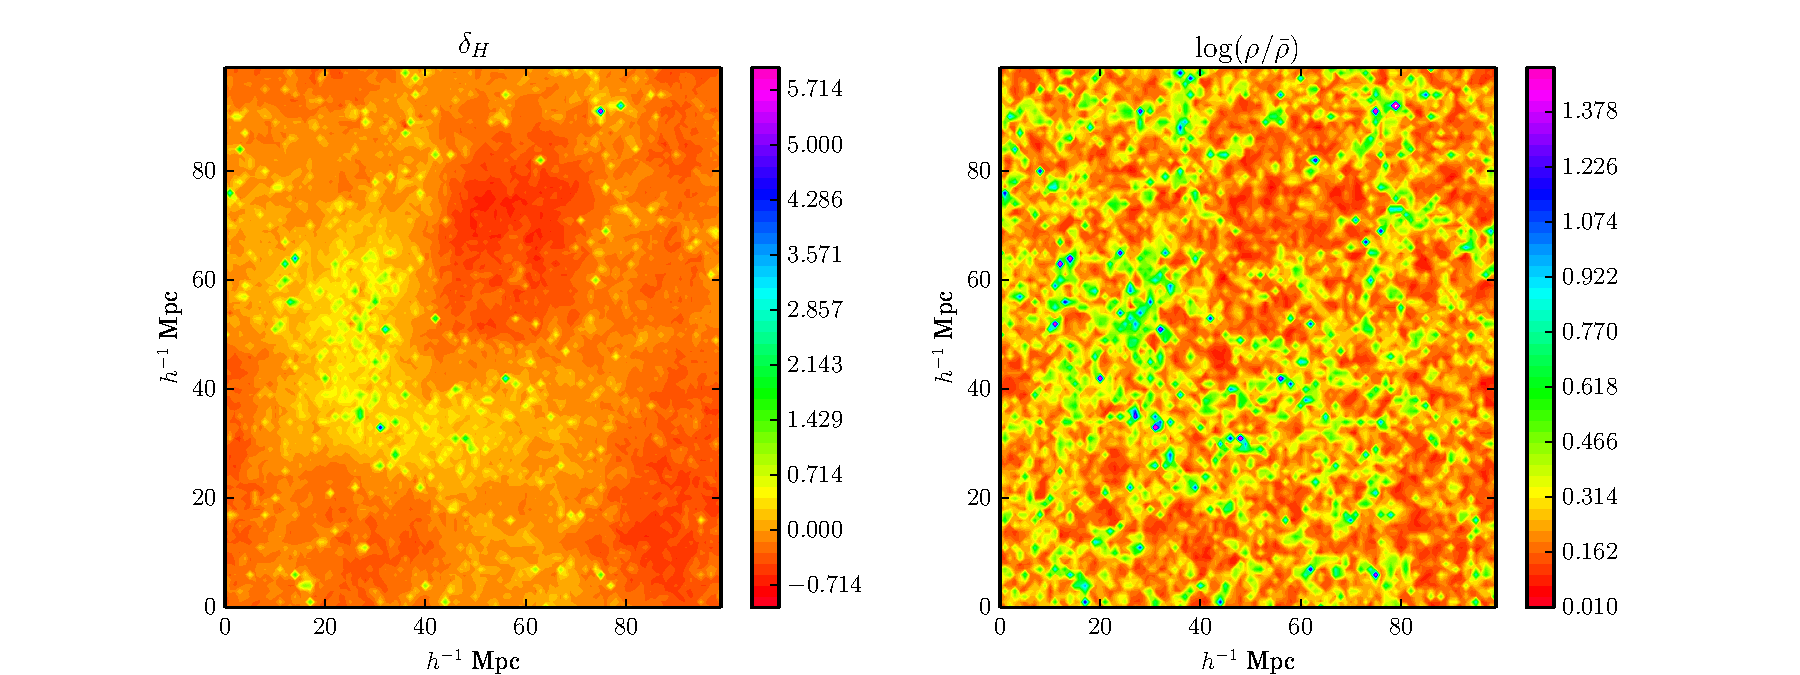
\includegraphics[width = .85\textwidth ]{data_delta_z4_256.pdf}
  % 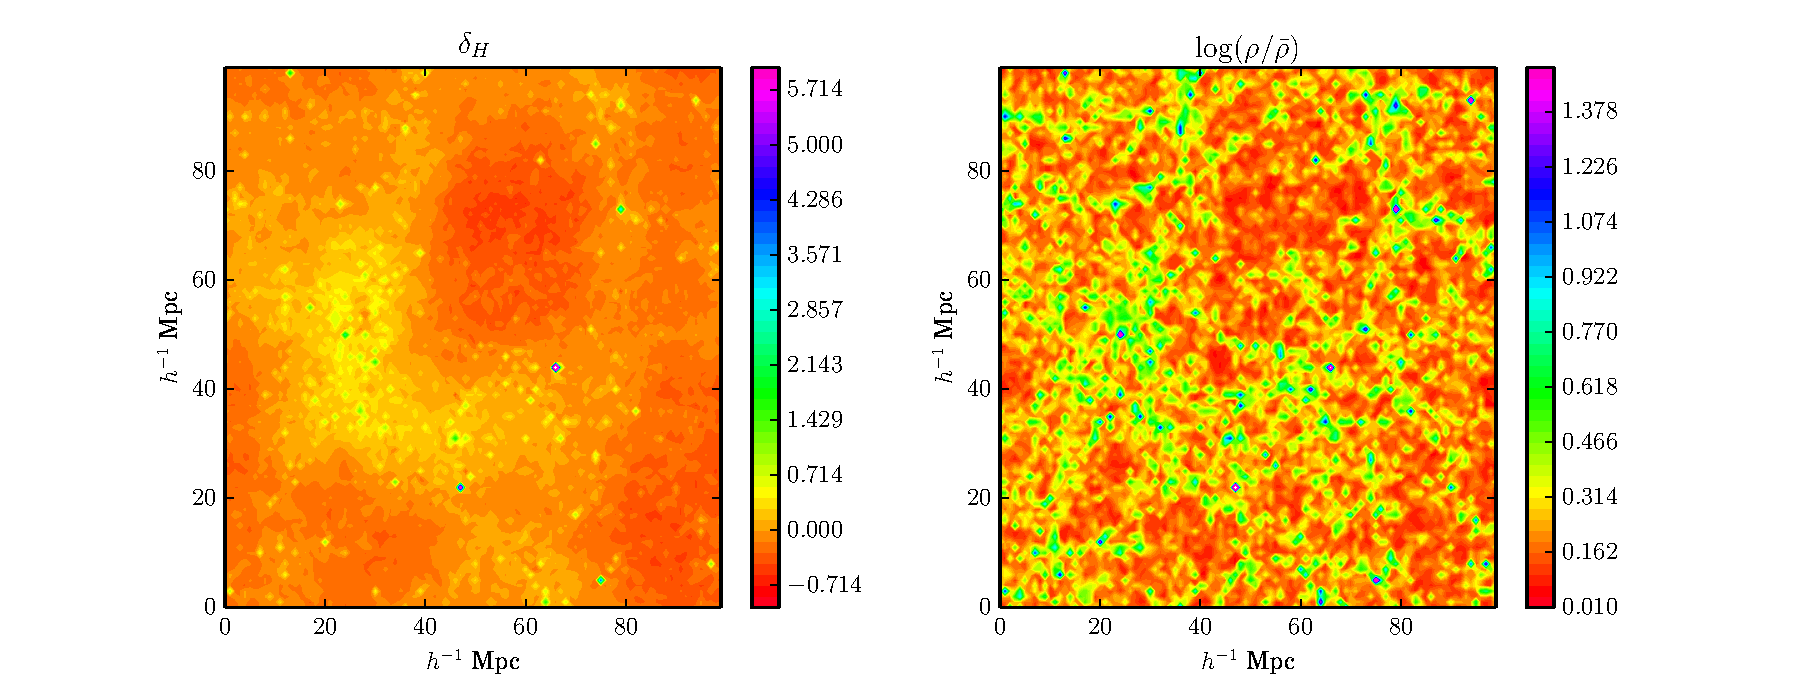
\includegraphics[width = .85\textwidth ]{data_delta_z3_256.pdf}
  % 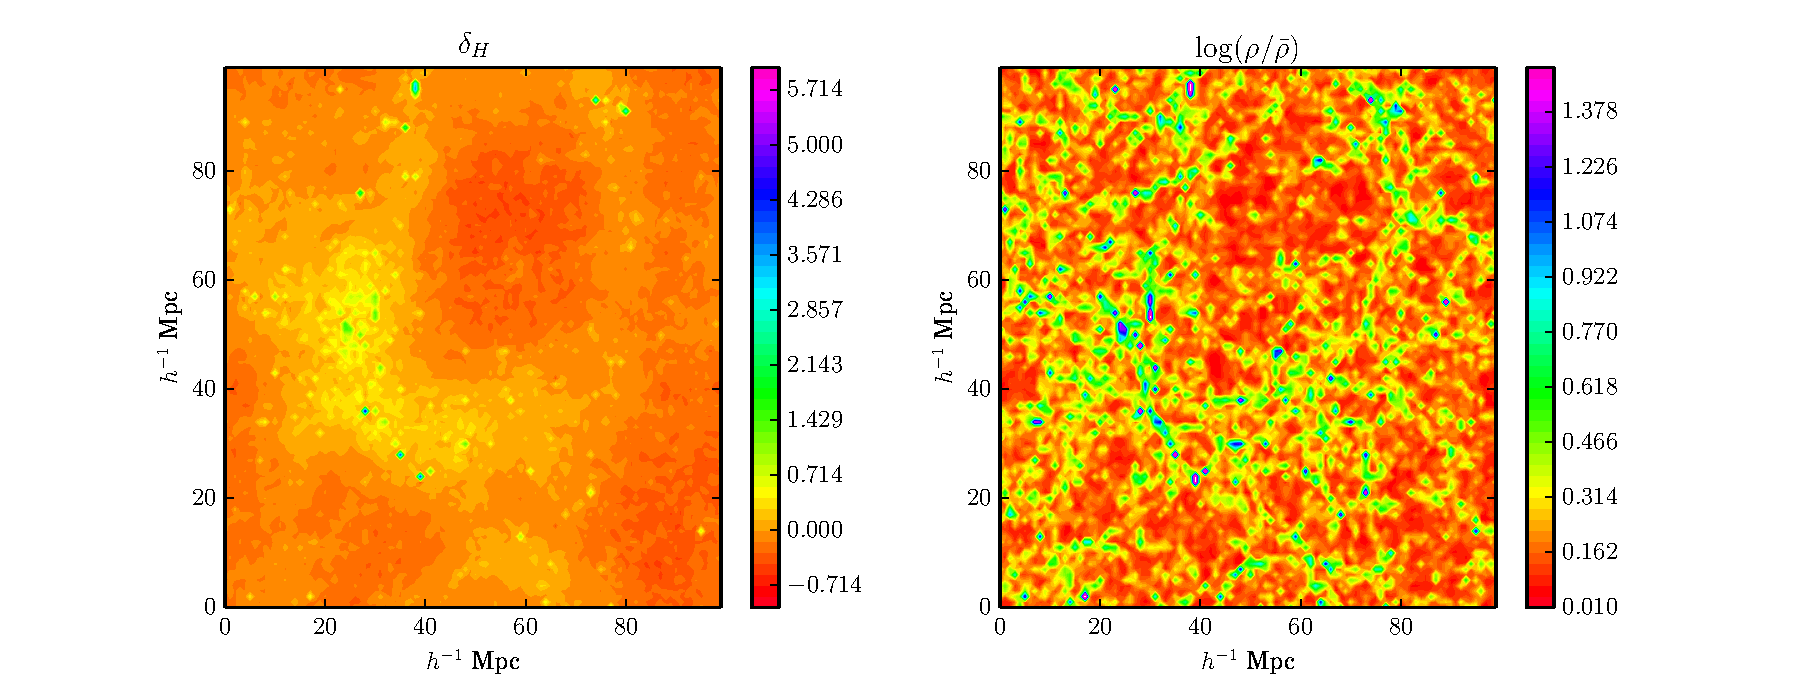
\includegraphics[width = .85\textwidth ]{data_delta_z2_256.pdf}
  % 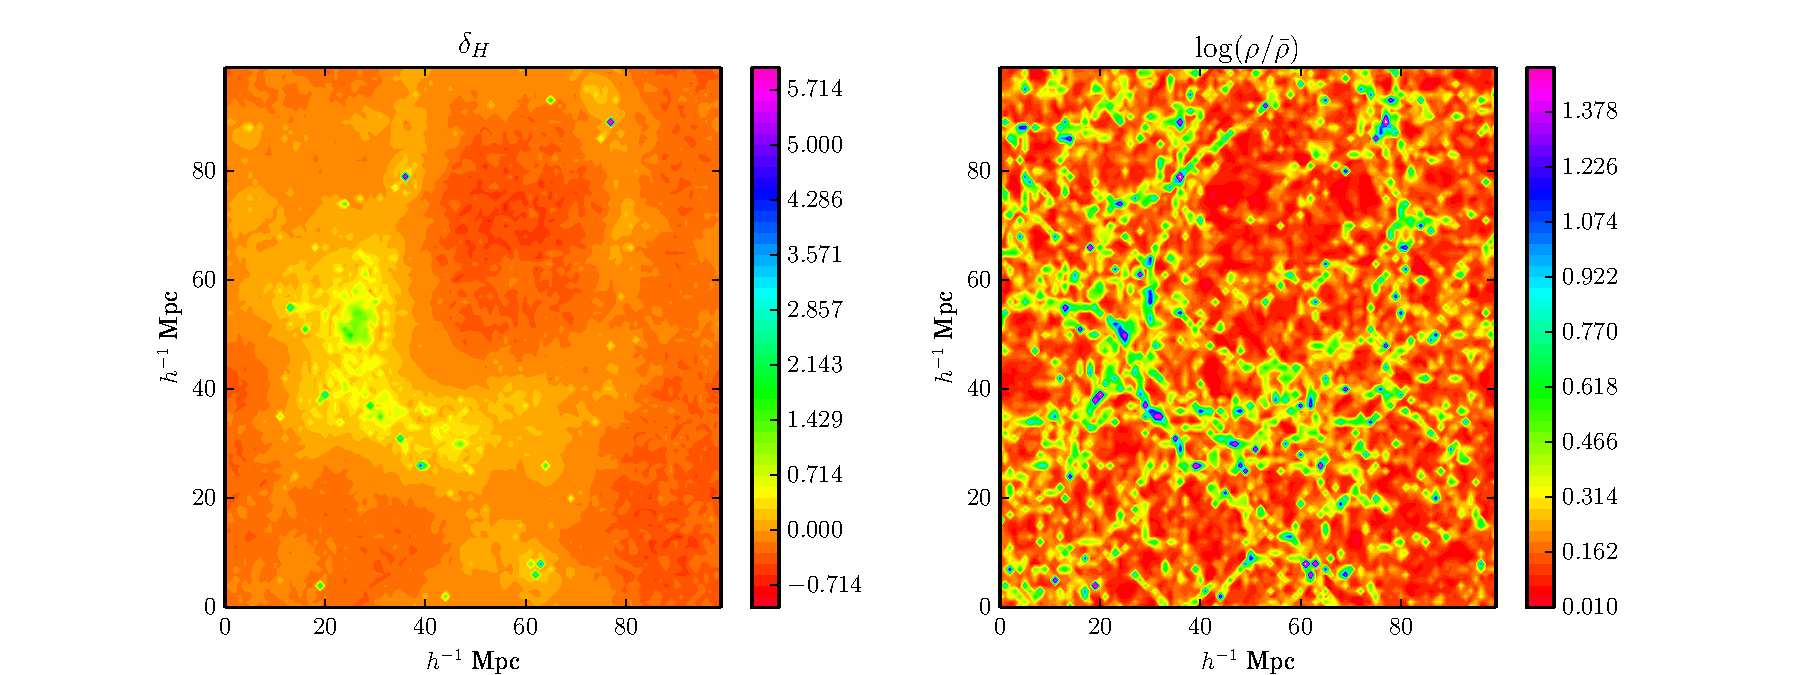
\includegraphics[width = .85\textwidth ]{data_delta_z1_256.pdf}
\includegraphics[width = .45\textwidth ]{data_rho_z3_qso4.png}
\includegraphics[width = .45\textwidth ]{data_rho_z1_qso4.png}
\includegraphics[width = .45\textwidth ]{data_delta_z3_gal2.png}
\includegraphics[width = .45\textwidth ]{data_delta_z1_gal2.png}

\includegraphics[width = .45\textwidth ]{data_delta_z3_qso4.png}
\includegraphics[width = .45\textwidth ]{data_delta_z1_qso4.png}

   \caption{ \ALc{Logarithm of the density with respect to the mean value (upper row), heating rate fluctuations with the galaxy (middle row) and quasar model  in the midplane of the box. The left column shows $z=3$, the right one $z=1$. }}
  \label{fig:slice}
\end{figure*}

\begin{figure*}
  \centering
%  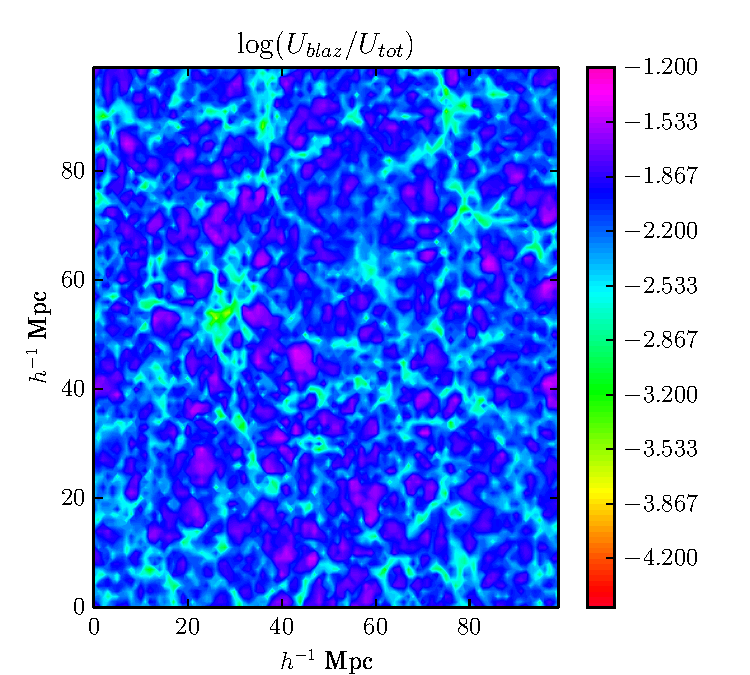
\includegraphics[width = .4\textwidth ]{data_U_z4_256.pdf}
%  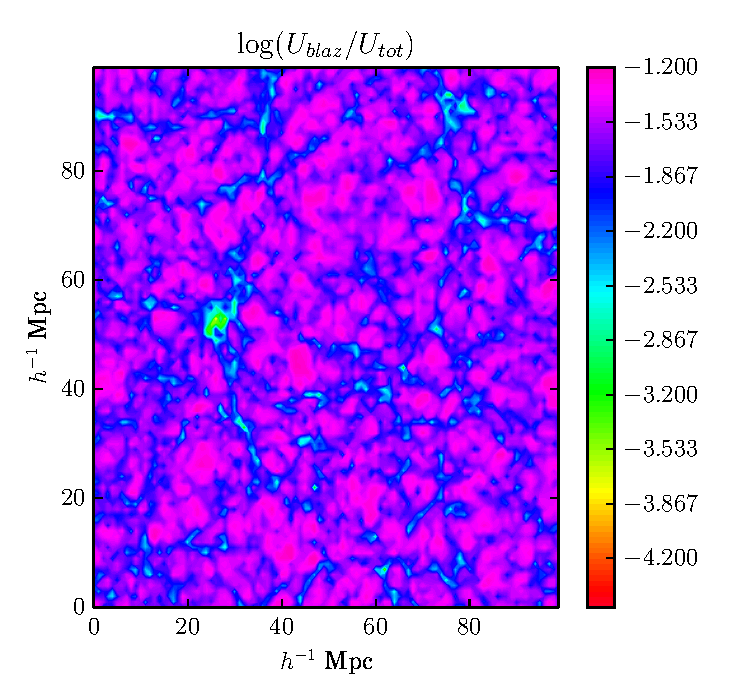
\includegraphics[width = .4\textwidth ]{data_U_z3_256.pdf}
  \includegraphics[width = .45\textwidth ]{data_U_z3_gal2.png}
  \includegraphics[width = .45\textwidth ]{data_U_z1_gal2.png}

  \includegraphics[width = .45\textwidth ]{data_U_z3_qso4.png}
  \includegraphics[width = .45\textwidth ]{data_U_z1_qso4.png}
   \caption{Ratio between the energy injection due to blazar heating and the total internal energy \ALc{the galaxy bias model (top) and the quasar bias model (bottom) for $z=3$ (left) and $z=1$ (right).}}
  \label{fig:heating_ratio}
\end{figure*}


Fig. \ref{fig:slice} shows the heating rate fluctuations in the midplane of the $L_x=100$ Mpc simulation for $z=3,1$ \ALc{for both the galaxy and quasar bias model}.  The corresponding density field is shown in the upper column and shows increasing structure formation as the redshift decreases.  The heating map has a linear scale while the density scale is logarithmic. The heating rate fluctuations are, on average, much smaller than the density fluctuations. This is because the window function filters out small scales, which correspond to collapsed regions,  where density fluctuations are the highest. To the zeroth order, one can thus consider TeV blazar heating to be uniform, as was assumed in PaperI.



Additional heating (i.e. $\delta_H>0$) occurs around clustered regions. This is expected, as the window function translates large scale density fluctuations into heating rate fluctuations.  Conversely, underdense regions, such as the one around $\{x=60,y=70\}$ display below average heating as they are isolated from sources, which flux decreases as $r^{-2}$. As the redshift decreases, heating rate fluctuations increase, following increasing density fluctuations.

Fig. \ref{fig:heating_ratio} shows the ratio of the internal energy due to  blazar heating with respect to the total internal energy.  These maps clearly highlight that blazar heating has more impact in underdense regions, as the heating rate per baryon is higher. Even if these regions receive less heat than regions with higher density (see Fig.~\ref{fig:slice}), blazar heating can account to up to $10\%$ of the total internal energy, especially in the quasar bias model.  This effect increases with time, as structures grow, the dense regions get denser and the voids get less dense. The ratio between the blazar induced energy and total energy first increases over time and then decreases between $z=2$ and $z=1$.  This evolution is related to the blazar luminosity evolution, which peaks at $z=2$ (PaperI).
%temperature: integrated heating rate.

The impact of inhomogeneous heating translates into a more complex temperature density relation, as is shown on Fig.~\ref{fig:T_rho}. The colormap shows the mass weighted $T-\rho$ relation from our simulations and the grey contours show the case for uniform blazar heating  \ALc{with the same resolution \citep{2012MNRAS.423..149P}}. When clustering is taken into account, the temperature-density relation has a significant scatter for underdense regions \ALc{especially when we use the quasar bias model}. For the quasar bias model, this scatter results in the lower envelope of the temperature-density relation to change little from the case with no blazar heating.  However, the mode of the temperature is very close to the uniform blazar heated case. At $z=1$ the simulation with the galaxy bias model has a very similar outcome to the uniform model and  blazar heating can be considered as homogeneous, though the lower envelope sits at a lower temperature.  \ALc{\sout{The scatter decreases with redshift as all regions of the universe have been affected by at least on TeV blazar. The temperature shows the impact of blazars \textit{integrated} over time, and thus asymptotically tends to the uniform case. } In both models, deviations from the uniform case become significant at $z\leqslant 3$.}

% The simulation with the quasar bias model shows significant deviation from the uniform case, especially at lower redshifts. Simulations following the galaxy bias model have less scatter and are similar to the uniform case at low redshift. }

% Regions at the mean cosmic density have temperatures between $T=9000$K and $T=60000$K at z=3, with a the peak of the distribution around$ T=20 000$ K. }



Fig.~\ref{fig:PDF} shows the mass-weighted probability distribution functions of the temperature for all the simulations. \ALc{Temperature measures the integrated impact of TeV blazar heating over time}. The simulation with the quasar bias model shows significant deviation from the uniform case, especially at lower redshifts. Here the effect of the lower envelope is clear as their is a significant tail toward lower temperatures for $z \leqslant 3$. \ALc{The scatter is strong for the quasar bias mode, where the coldest zones have $T\simeq 10 000K$ while the warmest zones have $T\simeq 30 000K$ for $z=3$. Conversely, the warmest gas is only slightly warmer than the mode of the temperature. The probability distribution function clearly highlights the impact of clustering on TeV blazar heating.}

% For $z\leqslant 4$, inhomogeneous blazar heating results in a lower average temperature and a larger scatter than the uniform case. \textit{The uniform case has a higher resolution, so the differences between the curves might be related to the resolution. I will test how this plot evolves with resolution}.  


\begin{figure*}
  \centering
  \includegraphics[width = .42\textwidth ]{T_rho_z4_256_gal2.png}
  \includegraphics[width = .42\textwidth ]{T_rho_z4_qso_256_div4.png}
  \includegraphics[width = .42\textwidth ]{T_rho_z3_256_gal2.png}
  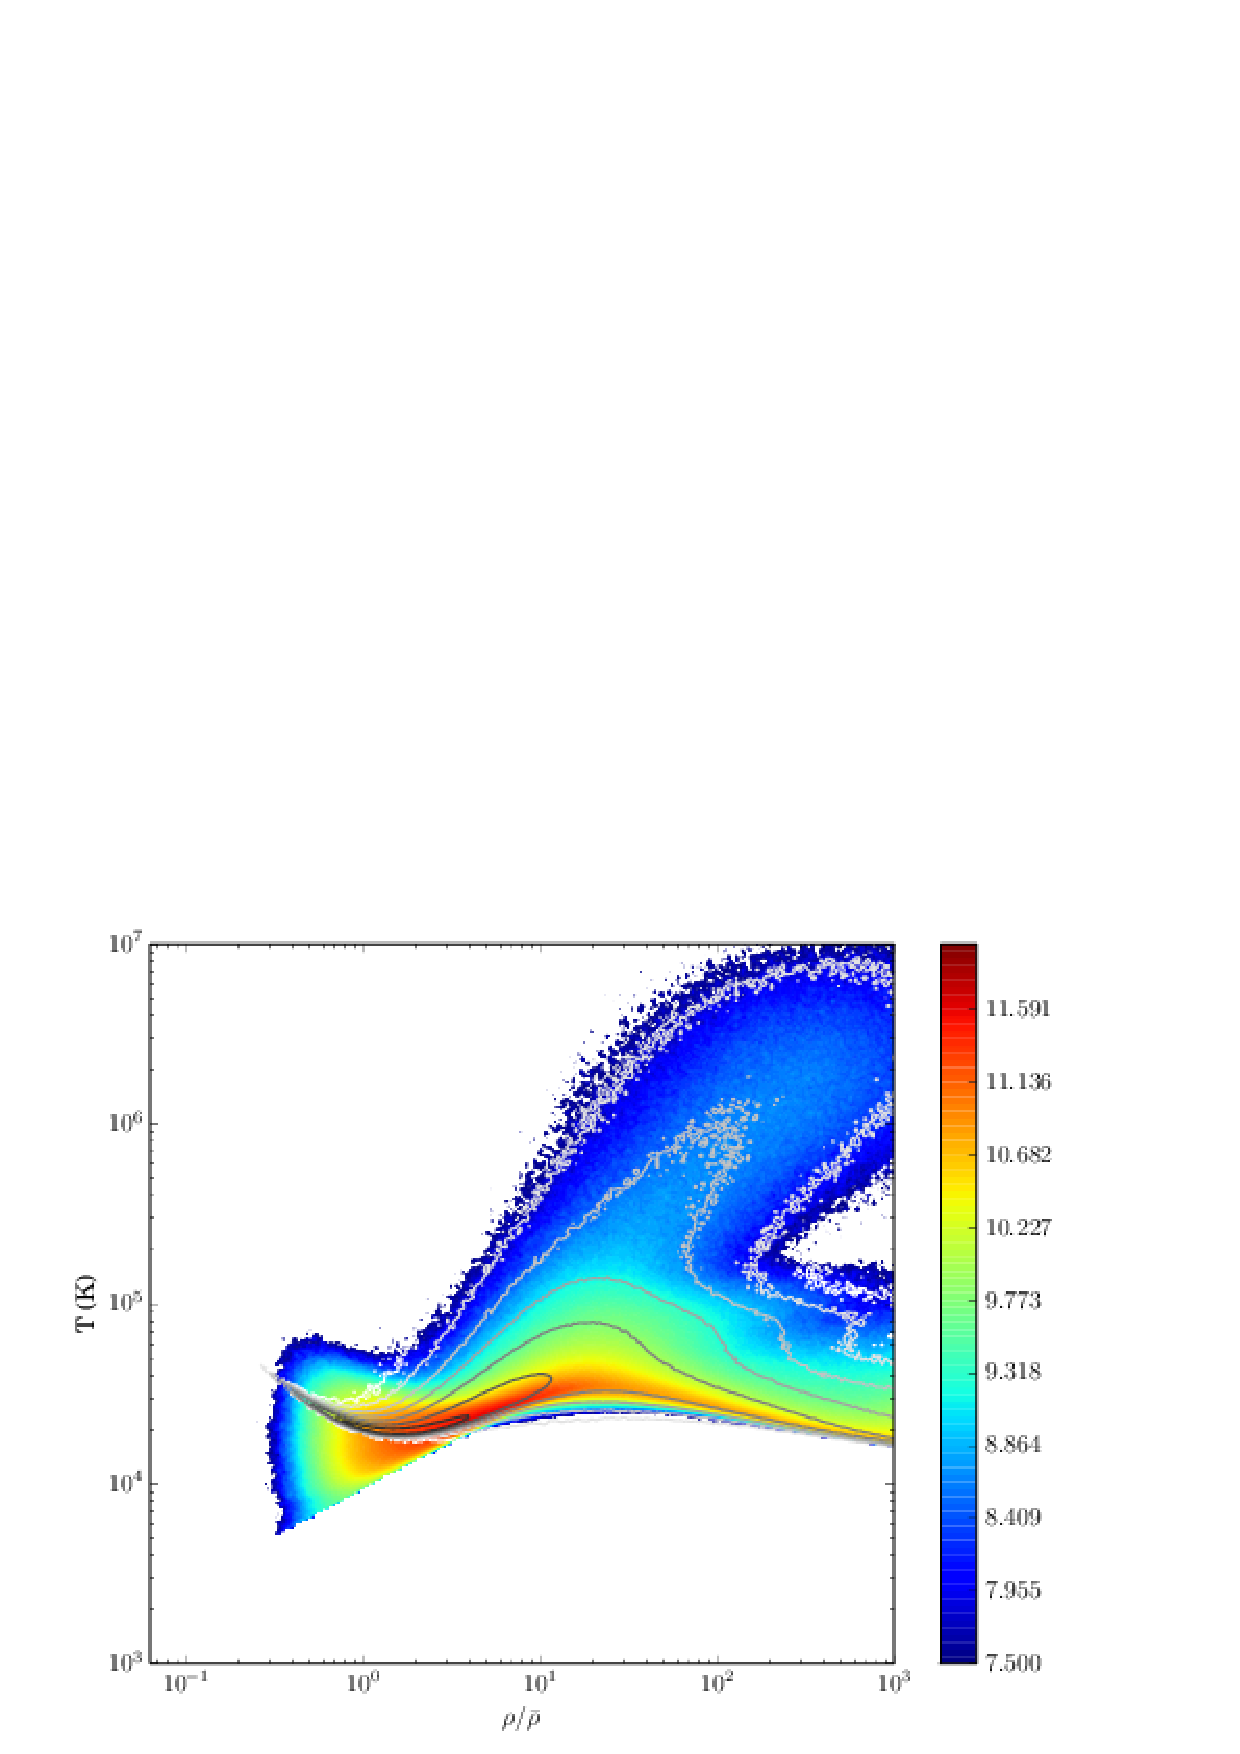
\includegraphics[width = .42\textwidth ]{T_rho_z3_qso_256_div4.png}
  \includegraphics[width = .42\textwidth ]{T_rho_z2_256_gal2.png}
  \includegraphics[width = .42\textwidth ]{T_rho_z2_qso_256_div4.png}
  \includegraphics[width = .42\textwidth ]{T_rho_z1_256_gal2.png}
  \includegraphics[width = .42\textwidth ]{T_rho_z1_qso_256_div4.png}
  \caption{Mass weighted temperature - density relation at $z=4,3,2,1$ (from top to bottom) for \ALc{the simulations with galaxy bias (left) and the quasar bias (right)} The overlying grey contours show the corresponding $T-\rho$ relation for uniform blazar heating \citep{2012MNRAS.423..149P} for the same mass range. }
  \label{fig:T_rho}
\end{figure*}


\begin{figure}[h]
  \centering
  \includegraphics[width = .45\textwidth ]{full_PDF_256_gal_qso.pdf}
%  \includegraphics[width = .42\textwidth ]{full_mass_PDF_256_gal_qso.pdf}
  \caption{Volume-weighted  temperature probability distribution function for $z=1$(black), 2 (blue), 3(cyan) and 4 (green) \ALc{for the quasar bias model (solid line), galaxy bias model (dashed line) and the uniform case (dotted line).} }
  \label{fig:PDF}
\end{figure}


To have a better understanding of the heating fluctuations with respect to density fluctuations we represent the mass-weighted  $\delta_H-\delta$ distribution on Fig. \ref{fig:deltas}. \ALc{The heating rate represents an instantaneous view of the impact of TeV blazar heating. In the quasar bias model (left rows), most of the particles receive slightly more heat than in the uniform case. However, the additional heat is only  a few times more than the uniform case. On the contrary, certain regions receive orders of magnitude less heat than the mean value. Certain areas suffer from the decrease of the TeV flux and isolation from massive structures. This is consistent with the temperature probability distribution function presenting an important low temperature tail and a low probability for high temperatures. In the galaxy model,  most of the gas has is heated similarly to the uniform case, translating the lower bias for galaxies.}


\begin{figure*}[h]
  \centering
  \includegraphics[width = .24\textwidth ]{delta_deltah_z3_qso4_256.png}
  \includegraphics[width = .24\textwidth ]{delta_deltah_z1_qso4_256.png}
  \includegraphics[width = .24\textwidth ]{delta_deltah_z3_gal2_256.png}
  \includegraphics[width = .24\textwidth ]{delta_deltah_z1_gal2_256.png}
\caption{Volume-weighted distribution of heating rate fluctuations $(1+\delta_H)$ with respect to the density fluctuations $(1+\delta)$ \ALc{\sout{for $z=4,3,2,1$ (from left to right)} for the quasar bias model (left columns) and the galaxy bias model (right columns) at $z=1$ (panel 1 and 3) and $z=3$ (panel 2 and 4). } The black dashed line represents the case of uniform blazar heating.}
  % \caption{Temperature (K), $\rho/\bar{\rho}$, heating rate fluctuations and contribution of blazar heating to the total internal energy.}
  \label{fig:deltas}
\end{figure*}



\ALc{
\section{Discussion}

In this paper, we have studied the impact of inhomogeneous TeV blazar heating on the IGM. Initial studies with spatially homogeneous heating \citep{2012ApJ...752...23C} indicated significant heating at $z\leqslant 3$, leading to an increased temperature of the intergalactic medium in low density regions. Including blazar heating in their simulations of the Lyman $\alpha$ forest, \citet{2012MNRAS.423..149P} find good agreement with observational data for the mean transmitted flux statistics as well as fits to individual lines.

Still, the lower envelope in the Lyman $\alpha$ linewidth as a function of column density indicates the presence of cold, unheated gas in the intergalactic medium at $z=2.4$ \citep{2012ApJ...757L..30R}. This suggests that, while most  of the IGM is heated up by TeV blazar heating, certain areas are too far from sources and remain unaffected.  In our simulations, which take into account clustering of the sources, we confirm the presence of such cold regions.  We find that, though most of the gas receives close to average heating, and has a temperature close to the uniform heating case, there is an important scatter in the temperature of the gas. If confirmed with the analysis of the resulting Lyman $\alpha$ forest, our model is able to account for both the observed increase in temperature in the low density IGM \citep{2014MNRAS.441.1916B,2009MNRAS.399L..39V} and the lower values  of the linewidths.

The impact of inhomogeneous heating becomes flagrant after $z=2.5$. At such redshift, the impact of HeII reionization  on the temperature of the IGM is  limited \citep{2013MNRAS.435.3169C}. An increased temperature, with a strong scatter in underdense regions can then be attributed to blazar heating. Such measurements are hard to obtain as the Lyman $\alpha$ forest is sensitive to overdensities of at least a few.  The Lyman $\alpha$ forest of HeII traces lower density regions and is a promising observable, with more data becoming available \citep{2014arXiv1405.7405W}.

A good understanding of the IGM is crucial as it is the birthplace of the large scale structures we observe. TeV blazar heating increases its average temperature and entropy, even at early times, and will impact the formation and evolution of  structures \citep{2012ApJ...752...24P}. Such heating occurs far away from the sources and  is complimentary to other black hole feedback mechanisms directly impacting their host galaxies and clusters.

\textit{ I am not totally sure about the next two paragraphs. If you have some references/thoughts about quasars vs blazars and issues like beaming and duty cycles, I'd like some comments here.}

Our model neglects important physical aspects of TeV blazars such as their duty cycle and  beaming of the gamma-ray emission. The  $\gamma$-ray duty cycle of BL Lac objects is of order of 10 $\%$ \citep{1996ApJ...464..600S}.  As TeV blazars have low accretion rates, their lifetime is long $\simeq 5-7$ Gyr \citep{2002ApJ...571..226C}.  The $\gamma$ ray sources are highly beamed, with observed opening angles peaking around 20$^{\circ}$ \citep{2009A&A...507L..33P}.  Parsec scale VLBI observations of the inner parts of radio jets indicate variations of the position angle of around 20$^{\circ}$, up to 120$^{\circ}$ over more than a decade \citep{2013AJ....146..120L}.   Both the beaming and small duty cycle yield extra variability in the distribution of the sources.   If the number  of sources of a given point is large, the variability of the source will be averaged out. However, when little sources are present, as in the early universe, individual variability increases the variability of blazar heating. In such case, our model is a lower limit for the associated heating rate fluctuations.

We test for two models for the bias, massive galaxies and quasars while BL Lacs are associated with giant elliptical galaxies \citep{2007A&A...476..723H}.  In the early universe, high gas density and mergers drive strong accretion, thus leading to quasar type accretion. Lower rates of accretion, i.e, blazar-type accretion,  is  are probably favoured in less dense environments. In this case, galaxy bias likely is a better representation for the bias of TeV sources. Later on, the available quantity of gas decreases, and giant elliptical occupy the high density central regions of clusters. In this case, TeV-photon sources are associated with the large scale high density regions and quasar bias is probably a better model for the bias. In our simulations, any dense source emits TeV photons, regardless of the type of galaxy, and history of merger and accretion.  However, a more detailed physical model, which comes at high computational cost, will very likely remain within those two limiting cases. The difference in the median temperature for both cases is less than $10\%$  and the standard deviation varies by XXXXX.



}


 



\begin{itemize}
\item linear assumption
\item assumption on EBL
\item suggest possible applications for window function
%\item BOSS
\item impact of shot noise
\end{itemize}

Detailed modeling of the spectral energy distribution of TeV blazars has enabled to measure the imprint of the EBL and partially  constrain its spectrum \citep{2013A&A...550A...4H}. The EBL is the sum of all the stellar and non-stellar emission throughout the history of the universe and carries important information on the total star formation. Due to strong foreground emission, direct measurements of the EBL are limited to lower limits \citep{2006A&A...451..417D}. 

\section{Conclusions}
\ALc{We have implemented inhomogeneous TeV blazar heating into cosmological simulations to study the impact of clustering on the thermal state of the intergalactic medium. Initial studies with spatially homogeneous heating \citep{2012ApJ...752...23C} indicated significant heating at $z\leqslant 3$, leading to an increased temperature of the intergalactic medium in low density regions. Including blazar heating in their simulations of the Lyman $\alpha$ forest, \citet{2012MNRAS.423..149P} find good agreement with observational data for the mean transmitted flux statistics as well as fits to individual lines.

Still, the lower envelope in the Lyman $\alpha$ linewidth as a function of column density indicates the presence of cold, unheated gas in the intergalactic medium at z=2.4 \citep{2012ApJ...757L..30R}.This suggests that, while most of the IGM is heated up by TeV blazar heating, certain areas are too far from sources and remain unaffected.  In this work, we extended the initial work and modeled the spatial fluctuations of blazar heating. 

We developed a filtering function relating heating rate fluctuations to the linear dark matter fluctuations, in Fourier space. Using this window function, we are able model the relevant lengthscales for the blazar heating fluctuations and include them in a statistical fashion. Our method is a cost effective alternative method to fully self consistent simulations of blazar heating where modeling black hole formation and growth and complete radiative transfer would have been prohibitive. 

Using this model for heating fluctuations, we find that large underdense regions receive less than one percent of the average heating rate while highly clustered regions receive up to five times more than the average heating rate at $z=1$. Still, as in the uniform case, the impact of TeV blazar heating is the strongest in low density regions. In our simulations, the mode of the temperature of the IGM is very close to the value in the uniform model, indicating the uniform model is a good zero-th order approximation. However, the temperature density relations we obtain present a much larger scatter than the uniform case, especially at low redshift. In our quasar bias model, the temperature at mean density varies by an order of magnitude between the coldest and warmest regions. 

Our model for the blazar heating fluctuations yields a temperature density relation which can potentially reconcile the observed increased mean temperature of the IGM \citep{2014MNRAS.441.1916B}, while maintaining a fraction of cold gas, responsible for the lower envelope of the linewidth distribution \citep{2012ApJ...757L..30R}. Therefore, detailed modeling of the Lyman $\alpha$ forest will be the subject of a forthcoming paper. If confirmed, this will clearly indicate a more complex  thermal history of the IGM, with potentially an important impact on late forming structures. 

}

\begin{acknowledgements}
This work was supported by the UWM Research Growth Initiative and NSF grant AST-1255469. Simulations were performed using HPC resources from TACC (Grant TG-AST 130004). \ALc{Add other grants here. Add Pleiades allocation as well.}
\end{acknowledgements}


\appendix

We detail the derivation of the window function in Eq. \ref{eq:window}. We start from a purely Newtonian universe, then include the impact of expansion and finally various first order corrections to the received TeV flux.
\section {Newtonian case}\label{sec:windon_newt}

\subsection {Fluctuations with respect to the mean heating rate}

The TeV flux received (in photons s$^{-1}$ cm$^{-2}$) at position $\mathbf{x}$ is given by the sum over all the sources within a radius $r\leqslant r_{max}$.
\begin{equation}
  \label{eq:flux_recu0}
  J(\mathbf{x})=\int_{0}^{2\pi}\int_{0}^{\pi}\int_0^{r_{max}}   \frac{\mathcal{E}(\mathbf{x}') }{4\pi |\mathbf{x}'-\mathbf{x}|^2} e^{-\tau} |\mathbf{x}'-\mathbf{x}|^2 \sin\theta d\theta d\phi d(\mathbf{x}'-\mathbf{x}),
\end{equation}
where the emissivity $\mathcal{E}$ is given in photons per unit time, per unit volume. $\tau=\kappa (\mathbf{x}'-\mathbf{x})$ is the optical depth along the line of sight, $\kappa$ the absorption coefficient.
Introducing $\mathbf{r'}=\mathbf{x}'-\mathbf{x}$, and $d\Omega=sin\theta d\theta d\phi$ this gives


\begin{equation}
  \label{eq:flux_recu}
  J(\mathbf{x})=\int_{\Omega}\int_0^{r_{max}}   \frac{\mathcal{E}(\mathbf{r}'+\mathbf{x}) }{4\pi } e^{-\tau} d\Omega dr'.
\end{equation}

The corresponding heating rate (erg cm$^{-3}$ s$^{-1}$ ) is given by 
\begin{equation}
  \label{eq:heating_rate0}
  \dot{Q}(\mathbf{x})=\frac{E_0}{D_{pp}}J(\mathbf{x}) =\frac{E}{4\pi}   \int_{\Omega}d\Omega\int_0^{r_{max}}   \mathcal{E}(\mathbf{r}'+\mathbf{x}) \frac{1}{D_{pp}}  e^{-\tau} dr' ,
\end{equation}
with $E_0$ the mean energy of the TeV photons and $D_{pp}$ their mean free path  before they pair-produce. For convenience reasons,  we  do not take into account the impact of the spectral energy distribution of the TeV photons in this Appendix. It is taken into account in the exact computation in section \S\ref{window}.

This gives the  heating rate per baryon
\begin{equation}
  \label{eq:heating_rate0}
  \dot{q}(\mathbf{x})=\frac{\dot{Q}}{n}= \frac{E_0}{4\pi}  \int_{\Omega}\int_0^{r_{max}}   \mathcal{E}(\mathbf{r}'+\mathbf{x})\sigma  e^{-\tau}d\Omega dr' ,
\end{equation}
where $n$ is the average density of the target photons (i.e. the EBL) and $\sigma$ (in cm$^{-2}$) is the energy averaged cross section for pair production on the extragalactic background light (EBL) photons \citep{1967PhRv..155.1408G}. 


The mean heating rate can be expressed as
\begin{equation}
  \label{eq:heating_rate0}
  \bar{\dot{q}}=\frac{E_0}{4\pi} \int_{\Omega}d\Omega\int_0^{r_{max}}  \bar{\mathcal{E}}\sigma  e^{-\tau}dr', 
\end{equation}
with $\bar{\mathcal{E}}$ the mean emissivity. Throughout the whole appendix, barred quantities are spatially averaged quantities.

The heating rate fluctuations at a given point are then given by 

\begin{eqnarray}
  \label{eq:heat_fluc_newt0}
  \delta_H(\mathbf{x})&=&\frac{\dot{q}(\mathbf{x})-\bar{\dot{q}}}{\bar{\dot{q}}}=\frac{E_0}{4\pi\bar{\dot{q}}} \int_{\Omega}d\Omega\int_0^{r_{max}}   (\mathcal{E}(\mathbf{r}'+\mathbf{x})-\bar{\mathcal{E}}) \sigma  e^{-\tau} dr' \\ \nonumber
  &=&\frac{E_0}{4\pi\bar{\dot{q}}}\int_{\Omega}d\Omega\int_0^{r_{max}}   \delta_E(\mathbf{r}'+\mathbf{x})\bar{\mathcal{E}}\sigma  e^{-\kappa r'}dr',
\end{eqnarray}
with the fluctuations in the TeV emissivity $\delta_E$ such that one has $\delta_E=\delta$ if the emissivity is directly related to the density.
% \begin{equation}
%   \label{eq:fluc_emissivity}
%   \delta_E(\mathbf{r}'+\mathbf{x})=\frac{\mathcal{E}(\mathbf{r'}+\mathbf{x})-\bar{\mathcal{E}}}{\bar{\mathcal{E}}}.
% \end{equation}



\subsection{Window function}
As the universe is infinite and asymptotically flat, we can expand the fluctuations into planar waves, in order to get the lengthscale dependence of heating rate fluctuations \citep{2004MNRAS.352..142B}.

\begin{eqnarray}
  \label{eq:FT_delta}
  \delta_H(\mathbf{x})&=&\frac{1}{(2\pi)^3}\int_{-\infty}^{\infty} d^3\mathbf{k'} \tilde{\delta}_H(\mathbf{k'}) e^{-i\mathbf{k'}\cdot\mathbf{x}}\\ \nonumber
  \delta_E(\mathbf{r}'+\mathbf{x})&=&\frac{1}{(2\pi)^3}\int d^3\mathbf{k'} \tilde{\delta}_E(\mathbf{k'}) e^{-i\mathbf{k'}\cdot(\mathbf{r'}+\mathbf{x})},
\end{eqnarray}
Eq. \ref{eq:heat_fluc_newt0} then gives
\begin{eqnarray}
  \label{eq:heat_fluc_newt1}
\frac{1}{(2\pi)^3}\int_{-\infty}^{\infty} d^3\mathbf{k'} \tilde{\delta}_H(\mathbf{k'}) e^{-i\mathbf{k'}\cdot\mathbf{x}}&=&\frac{E_0}{4\pi\bar{\dot{q}}} \int_{\Omega}d\Omega\int_0^{r_{max}}  dr' \bar{\mathcal{E}}\sigma  e^{-\kappa r'}  \frac{1}{(2\pi)^3}\int d^3\mathbf{k'} \tilde{\delta}_E(\mathbf{k'}) e^{-i\mathbf{k'}\cdot(\mathbf{r'}+\mathbf{x})}.
\end{eqnarray}

% To illustrate the next step, we perform a Fourier transform on Eq.\ref{eq:FFT} 
% \begin{eqnarray}
%   \label{eq:left}
% \frac{\tilde(\delta)(k)}{(2\pi)^3}&=&\frac{1}{(2\pi)^3}\int d^3\mathbf{k'}\tilde{\delta}(\mathbf{k'}) \int d^3\mathbf{x} e^{i(\mathbf{k}-\mathbf{k}')\cdot \mathbf{x}} \\
%  &=&  \frac{1}{(2\pi)^3}\int d^3\mathbf{k}'\delta^{(0)}(\mathbf{k}-\mathbf{k}')\tilde{\delta}_H(\mathbf{k}')\\
%   &=&  \frac{1}{(2\pi)^3} \tilde{\delta}_H(\mathbf{k})
% \end{eqnarray}




Performing an inverse Fourier transform on the right-hand side of Eq.\ref{eq:heat_fluc_newt0}, we have
\begin{eqnarray}
  \label{eq:right}
  &=& \frac{1}{(2\pi)^3} \frac{E_0}{4\pi\bar{\dot{q}}}\int_{\Omega}d\Omega\int_0^{r_{max}} dr'\bar{ \mathcal{E}}\sigma  e^{-\kappa r'} \int d^3\mathbf{k'}\int d^3\mathbf{x} \tilde{\delta}_E(\mathbf{k'})e^{-i\mathbf{k'}\cdot{\mathbf{r}'}} e^{i(\mathbf{k}-\mathbf{k'})\cdot\mathbf{x}} \\ \nonumber
  &=&\frac{1}{(2\pi)^3} \frac{E_0}{4\pi\bar{\dot{q}}} \int_{\Omega}d\Omega\int_0^{r_{max}}   dr' \bar{\mathcal{E}}\sigma  e^{-\kappa r'} \int d^3\mathbf{k'} \delta^{0}(\mathbf{k}-\mathbf{k}')e^{-i\mathbf{k'}\cdot{\mathbf{r}'}} \tilde{\delta}_E(\mathbf{k'})    \\ \nonumber
  &=&\frac{1}{(2\pi)^3} \frac{E_0}{4\pi\bar{\dot{q}}} \int_{\Omega}d\Omega\int_0^{r_{max}}  dr' \bar{ \mathcal{E}}\sigma  e^{-\kappa r'}  \tilde{\delta}_E(\mathbf{k}) e^{-i\mathbf{k}\cdot{\mathbf{r}'}}  ,
\end{eqnarray}
with $\delta^{(0)}$ the Dirac function, which Fourier transform equals 1. Introducing $\mu=cos\theta$, where $\theta$ is the angle between the wavevector and the line of sight, Eq. \ref{eq:heat_fluc_newt0} rewrites
\begin{eqnarray}
  \label{eq:heat_fluc_newt1}
  \tilde{\delta}_H(\mathbf{k})&=&  \frac{E_0}{\bar{2\dot{q}}} \int_{-1}^{1} d\mu \int_0^{r_{max}}  \bar{\mathcal{E}}\sigma  e^{-\kappa r'}  \tilde{\delta}_E(k) e^{-ikr'\mu}  dr'\\ \nonumber
&=&\tilde{\delta}_E(\mathbf{k})\frac{\sigma E_0}{\bar{\dot{q}}}\int_0^{r_{max}} \frac{sin(kr')}{kr'}   \bar{\mathcal{E}}  e^{-\kappa r'}   dr'\\ \nonumber
&=&\tilde{\delta}_E(\mathbf{k})\frac{\sigma E_0}{ \bar{\dot{q}}}\frac{\kappa}{k}  atan\left(\frac{k}{\kappa}\right)\\ \nonumber
&=&\tilde{\delta}(\mathbf{k})\frac{\sigma E_0}{ \bar{\dot{q}}}\frac{\kappa}{k}  atan\left(\frac{k}{\kappa}\right).\\ 
\end{eqnarray}

Fig.\ref{fig:window_newt} shows  window functions with different absorption coefficients in a purely Newtonian universe. The solid red line shows a case with no absorption, the dashed green line shows a case with $\kappa=10$ Mpc$^{-1}$.  In the former case, large scale sctructure has the strongest impact on heating, as larger regions have more sources. When absorption is present,  the impact of large scale structure (i.e. low k) remains constant as distant sources are absorbed. For scales equal to or larger than the cutoff, heating fluctuations follow density fluctuations and overdense regions get more heat. At smaller scales, the density structure has less impact on the heating, unless a strong overdensity is present.  

\begin{figure}
  \centering
  \includegraphics[width = .45\textwidth ]{newtonian_window}
  \caption{Window function for a non-expanding universe. The solid red line has very little absorption ($\kappa=10^{-5}$ Mpc$^{-1}$), the dashed green line has $\kappa=10 $ Mpc$^{-1}$ .}
  \label{fig:window_newt}
\end{figure}



\section{Expanding universe}\label{sec:window_exp}

We perform the same derivation as in the former section, replacing the integrals on the (comoving) distance by redshift integrals using
\begin{equation}
  \label{eq:proper_dist}
  dr=\int \frac{c}{H(z)} dz'.
\end{equation}
where  $H(z)$ is the Hubble parameter.

% The emissivity $\mathcal{E}$ is given in comoving units, while the heating rate  is expressed in proper units. The proper volume is  $(1+z)^3$ times larger than the comoving volume. 
%Let $\mathbf{s}$ a point with coordinates $(z,\theta,\phi)$, the heating rate at $\mathbf{s}$ is 

\begin{equation}
  \label{eq:int_exp_heat}
  \dot{q}(\mathbf{z})=\frac{E_0(1+z)^2}{4\pi}\int_{\Omega}d\Omega\int_z^{z_{max}}\frac{dl}{dz'}\sigma\mathcal{E}(E',z') e^{-\tau} dz'.
\end{equation}
 $z'=z+\Delta z$, with $\Delta z$ the difference in redshift between the emission and reception of the photons.

$\mathcal{E}(E',z')$ is  the   blazar luminosity at the energy $E'$,  which then redshifts to energy $E$ following 
\begin{equation}
  \label{eq:E_z}
  E'=E\frac{1+z}{1+z'}.
\end{equation}

$\tau(E,z',z)$ is the optical depth of a TeV photon observed at redshift $z$ with energy $E$, which was emitted at redshift $z'$ with energy $E'$.

\begin{equation}
  \label{eq:tau}
  \tau(E,z',z)=\int_z^{z'}dz''\frac{1}{D_{pp}}\frac{dl}{dz''}=\int_z^{z'}dz''\frac{c}{H(z'')}\frac{1}{D_{pp}},
\end{equation}



Similarly to Eq. \ref{eq:heating_rate0},  the mean heating rate is given by 
\begin{equation}
  \label{eq:mean_exp_heat}
  \bar{\dot{q}}=\frac{E_0(1+z)^2}{4\pi}\int_{\Omega}d\Omega\int \frac{dl}{dz'}\sigma\bar{\mathcal{E}} e^{-\tau}dz'.
\end{equation}
%\textit{Here I'm not quite sure about the boundaries for the integral. Should we integrate from z=0 to zmax? I'm also puzzled about what to do with the redshift of the energy.}

The resulting heating rate fluctuations are then given by

\begin{eqnarray}
  \label{eq:fluc_exp0}
  \delta_H(\mathbf{s})&=&\frac{\dot{q}(\mathbf{s})-\bar{\dot{q}}}{\bar{\dot{q}}}=\frac{E_0(1+z)^2c\sigma}{4\pi\bar{\dot{q}}} \int_{\Omega}d\Omega\int_z^{z_{max}} \frac{ ( \mathcal{E}(z')-\bar{\mathcal{E}})  e^{-\tau}}{H(z')} dz' \\ \nonumber
  &=&\frac{E_0(1+z)^2\bar{\mathcal{E}} c\sigma}{4\pi\bar{\dot{q}}}  \int_{\Omega}d\Omega\int_0^{z_{max}}   \frac{\delta_E(z')  e^{-\tau}}{H(z')}dz'.
\end{eqnarray}

The TeV emission is related to the presence of supermassive black holes at the center of galaxies, which are located in collapsed dark matter halos.  We can thus connect the fluctuations of the TeV emission, within a certain radius $r$, to the underlying dark matter fluctuations $\delta$.
% \begin{equation}
%   \label{eq:delta}
%   \delta(z,r)=\frac{\rho(z,r)-\bar{\rho}(z)}{\bar{\rho}(z)},
% \end{equation}

% where $\rho$ is the dark matter  density of the Universe. 

At this stage we assume the TeV fluctuations exactly match the dark matter fluctuations $\delta_E=\delta$.  We explain in the next section that this is not exactly true and will take into account various corrections.  The initial density fluctuations represent a Gaussian random field, which exact properties depend on the earliest stages of the Universe prior to recombination \citep{1986ApJ...304...15B,Peebles}. They grow linearly between $z'$ and $z$ following $\delta(z',r)=\delta_0(r)D(z')/D(z)$ \citep{ 1977MNRAS.179..351H}.

\begin{equation}
  \label{eq:growth_1}
  D(z)=D_0H(z)\int_z^{\infty}\frac{1+z'}{H^3(z')}dz'.
\end{equation}
%The dark matter fluctuations initially grow linearly as the different Fourier modes of $\delta(\mathbf{k})$ evolve at the same rate, independently. 
The linear approximation breaks down when the amplitude of the root mean square of the perturbations approaches unity. The evolution of the density field is then determined by the spherical collapse \citep{1972ApJ...176....1G} and the virialization of halos. As the growth of the modes is independent of the wavenumber, we have

\begin{equation}
  \label{eq:FT_delta}
  \delta_E(z',r)=\delta(z',r)=\delta_o(r)D(z')=\delta_0D(z')\frac{1}{(2\pi)^3}\int d^3\mathbf{k'} \tilde{\delta}(\mathbf{k'}) e^{-i\mathbf{k'}\cdot\mathbf{r}}.
\end{equation}


And Eq. \ref{eq:fluc_exp0}  rewrites as
\begin{equation}
  \label{eq:heat_fluc_exp0}
  \delta_H(\mathbf{s})=\frac{ E_0(1+z)^2 \bar{\mathcal{E}} c\sigma}{4\pi\bar{\dot{q}}} \int_{\Omega}d\Omega\int_z^{z_{max}}  \frac{D(z')}{D(z)} \frac{\delta(r') e^{-\tau}}{H(z')}dz'.
\end{equation}


The left hand side yields $\tilde{\delta}(\mathbf{k})$ while the right hand side transforms in a similar fashion to Eq. \ref{eq:right}. As the power spectrum of density fluctuations is isotropic, this  yields

\begin{equation}
  \label{eq:heat_fluc_exp1}
  \tilde{\delta}_H(k)=\tilde{\delta}(k) \frac{E_0(1+z)^2\bar{\mathcal{E}}c\sigma}{4\pi\bar{\dot{q}}} \int_z^{z_{max}} \frac{D(z')}{D(z)}\frac{sin(kr'(z'))}{kr'(z')}    \frac{e^{-\kappa r'(z')}} {H(z')}  dz'.
\end{equation}

\begin{figure}[h]
  \centering
  \includegraphics[width = .45\textwidth ]{window_nobiases}
  \caption{Window function in an expanding universe.}
  \label{fig:window_nobiases}
\end{figure}

Fig. \ref{fig:window_nobiases} shows the window function in an expanding universe at different redshifts.  %Comparing with non-expanding case in Fig. \ref{fig:window_newt} \textit{ blabla} 
The TeV emission fluctuations are not exactly equal to the dark matter density fluctuations. In the next section we will account for the various corrections that have to be taken into account to determine a more accurate window function.


\section{Complete window function}
 \ALc{
The TeV fluctuations are biased with respect to the dark matter fluctuations, as we detail in $\S$ \ref{sec:bias}, yielding 
\begin{equation}
  \delta_E=(1+b(z)\delta)
\label{eq:bias}
\end{equation}

On top of that, the emitting area (which corresponds to the proper area), evolves as
  \begin{equation}
    \label{eq:emitting_area}
4\pi r(z)^2=4\pi r^2\left(\frac{\bar{\rho}}{\rho(z)}\right)^{2/3}=4\pi r^2(\delta(z)+1)^{2/3}.
  \end{equation}
A small density perturbation thus gives
\begin{equation}
  \label{eq:pert_area}
dA\simeq 4\pi \left(1+\frac{2}{3}\delta\right)r^2.
\end{equation}

If galaxies were moving exactly with the Hubble flow, their redshift would yield their exact distance to an observer. However, galaxies galaxies bound to a central potential of a cluster have an infall velocity towards the central overdensity. The proper distance to a source  (Eq. \ref{eq:proper_dist}) then becomes

  \begin{equation}
    \label{eq:vel_perturb}
    dz'=dr\frac{H(z')}{c}\left(1-\frac{d\delta_{v_r}(z')}{dr}\right),
  \end{equation}
where $\delta_{v_r}$ are the velocity perturbations along the line of sight. The Fourier transform of $\delta_{v_r}$ gives  \citep{1987MNRAS.227....1K}.

\begin{equation}
  \label{eq:kaiser2}
  \mathcal{F}\left(\frac{d\delta_{v_r}}{dr}\right)=-\mu^2\tilde{\delta}(\mathbf{k}),
\end{equation}
with $\mu$ the cosine of the angle between the wavenumber and the line of sight.
}


%
%\subsection{Galaxy bias}
% \ALc{\sout{The TeV flux fluctuations are related to the distribution of galaxies, which is biased with respect to the distribution of dark matter halos, which in turn is biased with repect to the initial linear dark matter density fluctuations  \citep{1996MNRAS.282..347M}.  One defines the galaxy bias as the ratio between the power spectrum of galaxies to the power spectrum of the DM halos (see e.g. \citep{2002PhR...372....1C} for a review).  Galaxies bias is usually derived from simulations \citep{1999MNRAS.307..529K}, and observations for low redshifts \citep{2004ApJ...606..702T}. Galaxy bias is only weakly dependent on scale \citep{1998MNRAS.293..209M}, especially at low redshifts. Performing  a fit to Fig.9 in \citet{2004ApJ...601....1W}, we use $b_{gal}(z)=e^{0.4z}$. 
% }}



%The formation of galaxies within a certain halo relates to the possibility for the baryonic gas to cool, which is a highly complex astrophysical process. One defines the galaxy bias as the ratio between the power spectrum of galaxies to the power spectrum of the DM halos (see e.g. \citep{2002PhR...372....1C} for a review).  It is given by
% \begin{equation}
%   \label{eq:gal_bias}
%   b_{gal}=\int_{M_0}^{\infty} dM N(M) b(M) \frac{\langle N_{gal}|M\rangle }{\bar{n}_{gal}},
% \end{equation}
% where $N(M)$ is the halo mass distribution,  $\langle N_{gal}| M\rangle$ the number of galaxies contained in a halo of mass $M$ and $\bar{n}_{gal}$ the mean number of galaxies per halo. $b(M)$ is the halo bias, relating the halo distribution to the dark matter distribution \citep{1996MNRAS.282..347M}, such that the number of halos formed in a region of overdensity $\delta$ is given by

%   \begin{equation}
%     \label{eq:halo_bias}
%     N(M,\delta)=[1+b(M)\delta(z)]N(M).
%   \end{equation}

% $b$ has values of order unity, with increase at higher redshifts. This means that the denser regions of the Gaussian random field are more clustered than the regions with average density. Massive halos have a stronger bias, as they are not numerous.  In  our computation, the bias is mass-averaged over the halo Press-Schechter halo  mass distribution \citep{1999MNRAS.308..119S}.




%\subsection{Increased area}



%\subsection{Redshift-space distortions}

%\subsection{Window function }
Keeping only first order correction for density fluctuations, Eq.\ref{eq:int_exp_heat} yields
\begin{equation}
  \label{eq:mean_heat0}
  \dot{q}(\mathbf{s})=\frac{E_0(1+z)^2c\sigma\mathcal{\bar{E}}}{4\pi}\int_{\Omega}d\Omega\int_z^{z_{max}}\frac{D(z')}{D(z)}\left(1+\left(b(z)+\frac{2}{3}\right) \delta(r) -\frac{d\delta_{v_r}}{dr}\right) dz'.
\end{equation}

Substracting the mean heating rate (Eq. \ref{eq:mean_exp_heat}) then yields the fluctuations

\begin{equation}
  \label{eq:heat_fluc0}
  \delta_H(\mathbf{s})=\frac{1}{X}\int_{\Omega}d\Omega\int_z^{z_{max}}\frac{dX}{dz'}\frac{D(z')}{D(z)}\left(\left(b(z)+\frac{2}{3}\right) \delta(r) -\frac{d\delta_{v_r}}{dr}\right)   dz',
\end{equation}
where we introduced
\begin{equation}
  \label{eq:def_X}
  \frac{dX}{dz'}=\frac{E_0(1+z)^2\mathcal{\bar{E}}c\sigma}{4\pi}\frac{e^{-\tau(z,z',E')}}{H(z')},
\end{equation}
for convenience reasons and to highlight the generality of the method.


Switching to $k$-space then yields


\begin{eqnarray}
  \label{eq:heat_fluc0}
  \tilde{\delta}_H(k)&=&\frac{1}{X}\int_{\Omega}d\Omega\int_z^{z_{max}}\frac{dX}{dz'}\frac{D(z')}{D(z)}\left(\left(b(z)+\frac{2}{3}\right) \delta(\mathbf{r'}+\mathbf{x}) -\frac{d\delta_{v_r}(\mathbf{r'}+\mathbf{x})}{dr}\right)  dz'\\ \nonumber
&=&\frac{1}{X}\int_{\Omega}d\Omega\int_z^{z_{max}}\frac{dX}{dz'}\frac{D(z')}{D(z)}\Biggl((b(z)+\frac{2}{3}) \int d^3\tilde{\delta}(\mathbf{k})'\delta^{(0)}(\mathbf{k}-\mathbf{k'})e^{-i\mathbf{k}' \cdot \mathbf{r}'}\tilde{\delta}(\mathbf{k}')- \int d^3\mathbf{k}'e^{-\mathbf{k}'\cdot \mathbf{r}'}\delta(\mathbf{k}')\delta^{(0)}(\mathbf{k}+\mathbf{k}')\mu^2 \Biggr)  dz'\\ \nonumber
&=&\frac{\tilde{\delta}(\mathbf{k})}{X}\int_{-1}^{1}d\mu\int_z^{z_{max}}\frac{dX}{dz'}\frac{D(z')}{D(z)}\left((b(z)+\frac{2}{3})+\mu^2\right) e^{-ikr\mu}   dz'\\ \nonumber
&=&\frac{\tilde{\delta}(\mathbf{k})}{X}\int_z^{z_{max}}\frac{dX}{dz'}\frac{D(z')}{D(z)}\left((b(z)+1)j_0(kr)-\frac{2}{3}j_2(kr)\right)dz'.
\end{eqnarray}
With the spherical Bessel functions
\begin{eqnarray}
  \label{eq:bessel}
j_0(kr)&=&  \frac{sin(kr)}{kr}\\
j_2(kr)&=& \left(\frac{3}{x^2}-1\right)\frac{sin(x)}{x}-\frac{3 cos(x)}{x^2}  .
\end{eqnarray}
We have used

\begin{equation}
  \label{eq:bes2}
  \int_{-1}^{1}\mu^2 e^{i k r \mu} d\mu=\frac{2 sin(kr)}{kr}+4\frac{cos(kr)}{(kr)^2}-4\frac{sin(kr)}{(kr)^3}.
\end{equation}
The window function for the heating rate fluctuations is then given by 

\begin{equation}
  \label{eq:heat_fluc}
  \tilde{W}_H(k,z)=\frac{E_0(1+z)^2\sigma c \mathcal{\bar{E}}}{4\pi\bar{\dot{q}}}\int_z^{z_{max}} \frac{e^{-\tau}}{H(z')}\frac{D(z')}{D(z)}\left((b(z)+1)j_0(kr)-\frac{2}{3}j_2(kr)\right)dz'.
\end{equation}

Which is the same window function as  \citet{2007MNRAS.376.1680P,2005ApJ...626....1B}. 


\bibliographystyle{apj}
\bibliography{biblio_total}

 \end{document}
